\ifnum\printdraft>0
	Here goes specific results for Naïve bayes.
\else
\begin{center}
  	\textbf{--- DRAFT PARTS ---}
\end{center}
\fi
\newcommand{\figwidth}{0.45\textwidth}
\begin{figure}[H]
	\centering
	\begin{subfigure}[b]{\figwidth}
		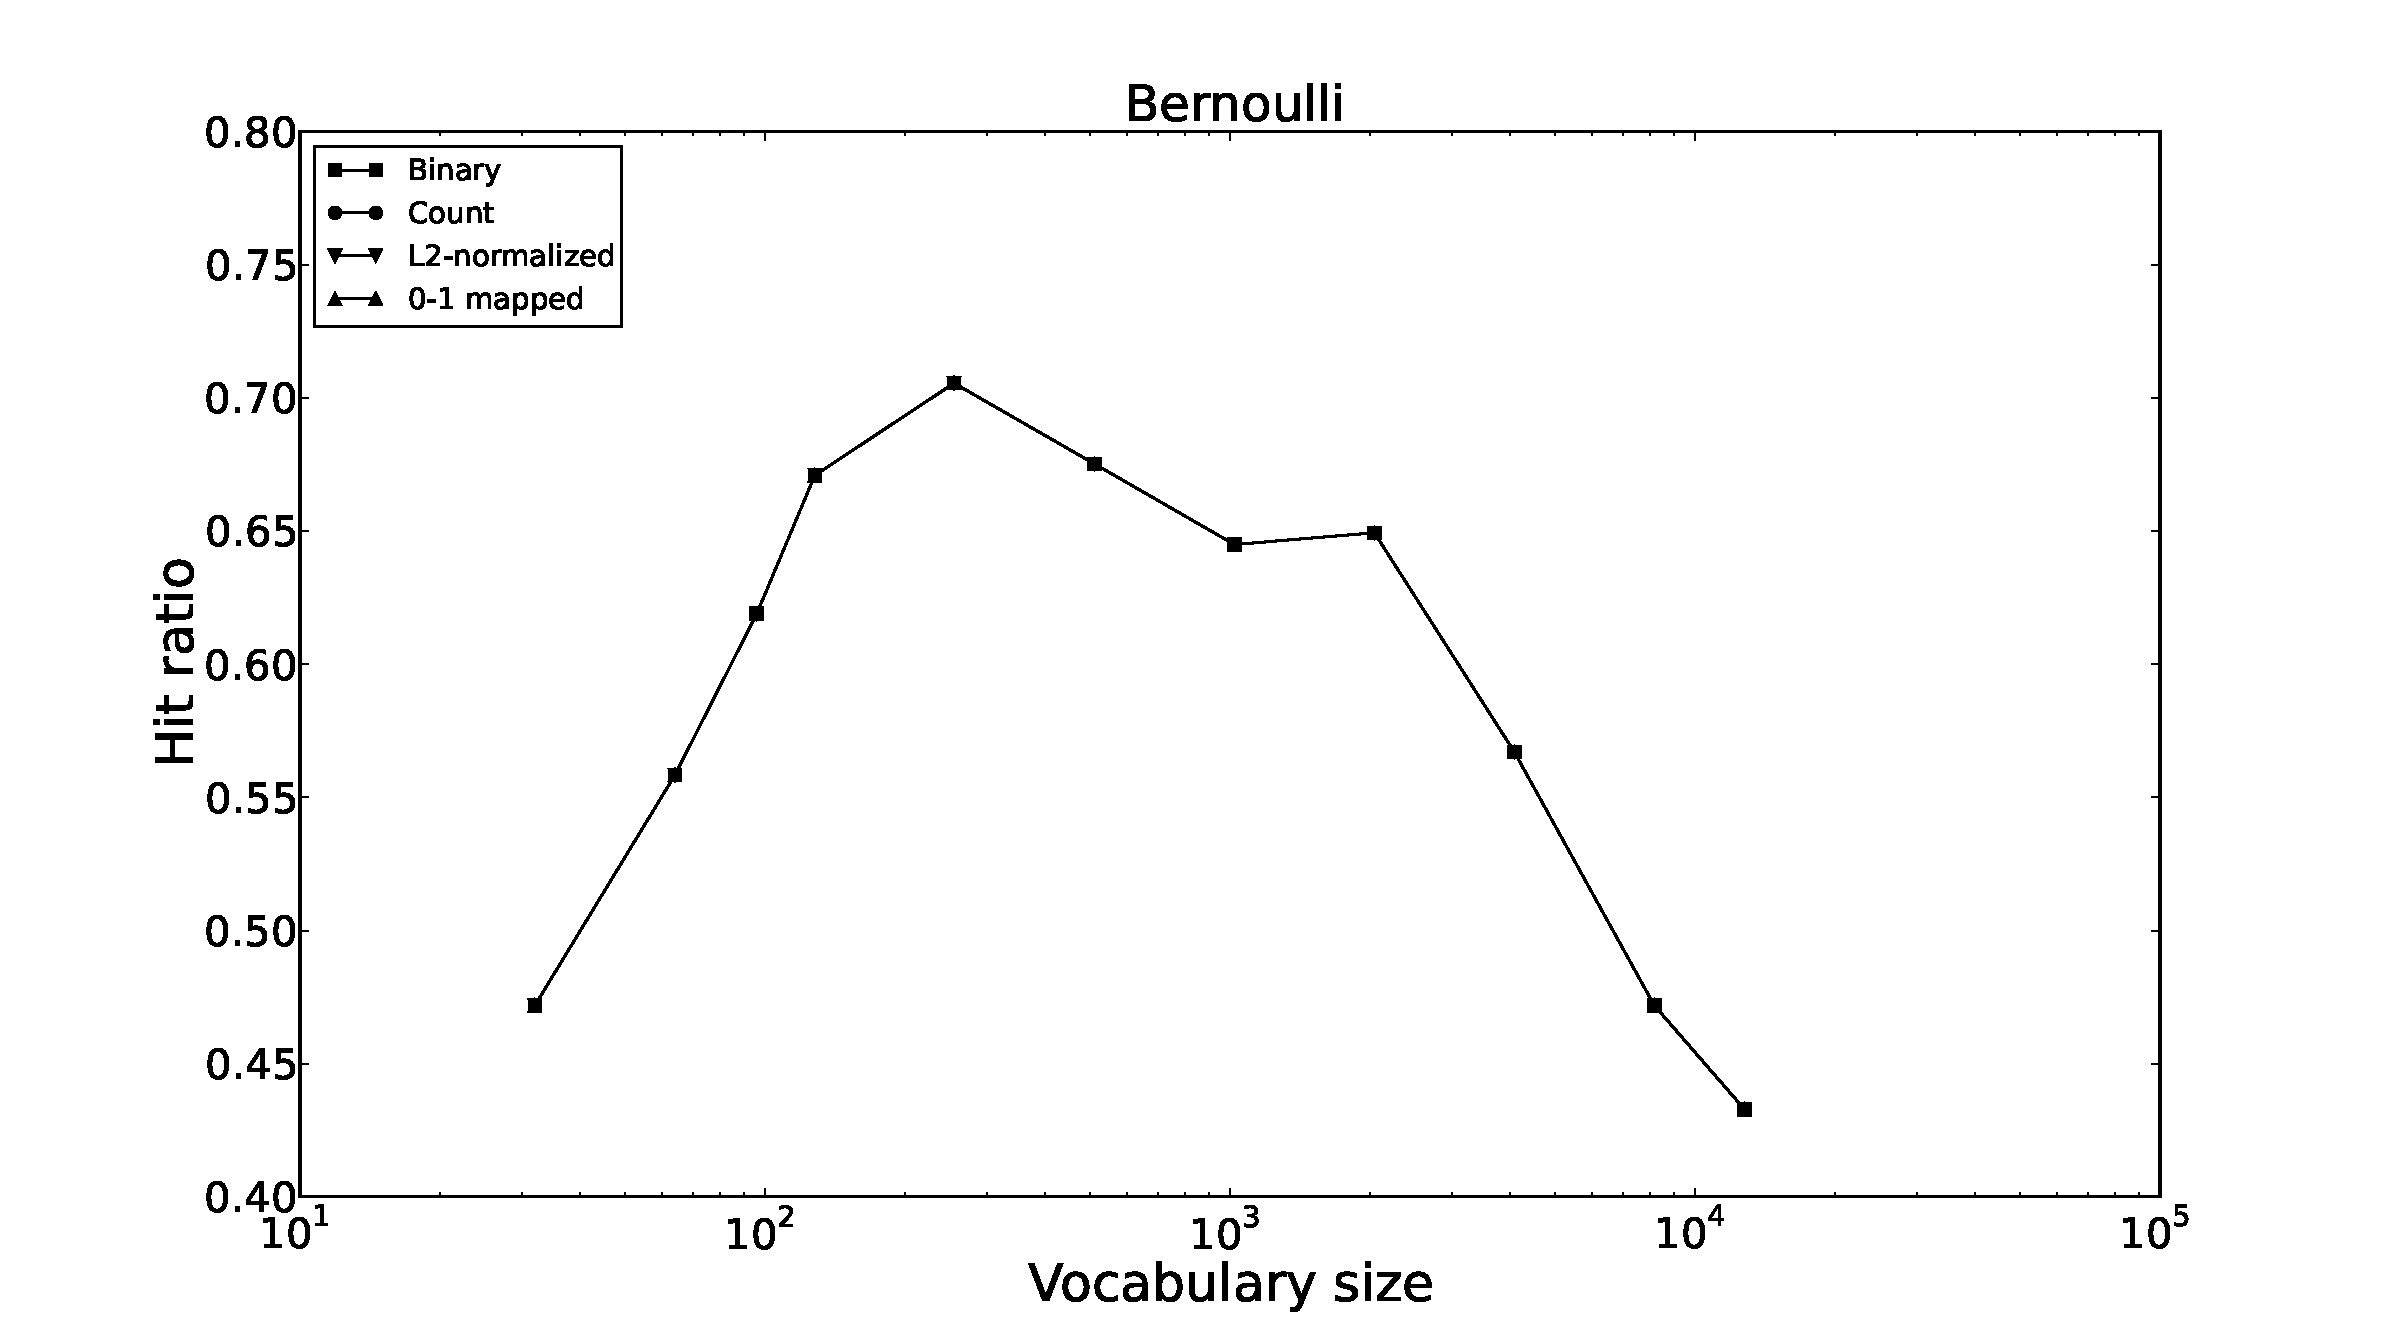
\includegraphics[width=\textwidth]{img/Bernoulli-hitrate-eps-converted-to.pdf}
		\caption{Hit ratio of Bernoulli classifier with varying vocabulary size.}
		\label{fig:hitrate-nb}
	\end{subfigure}
	~
	\begin{subfigure}[b]{\figwidth}
		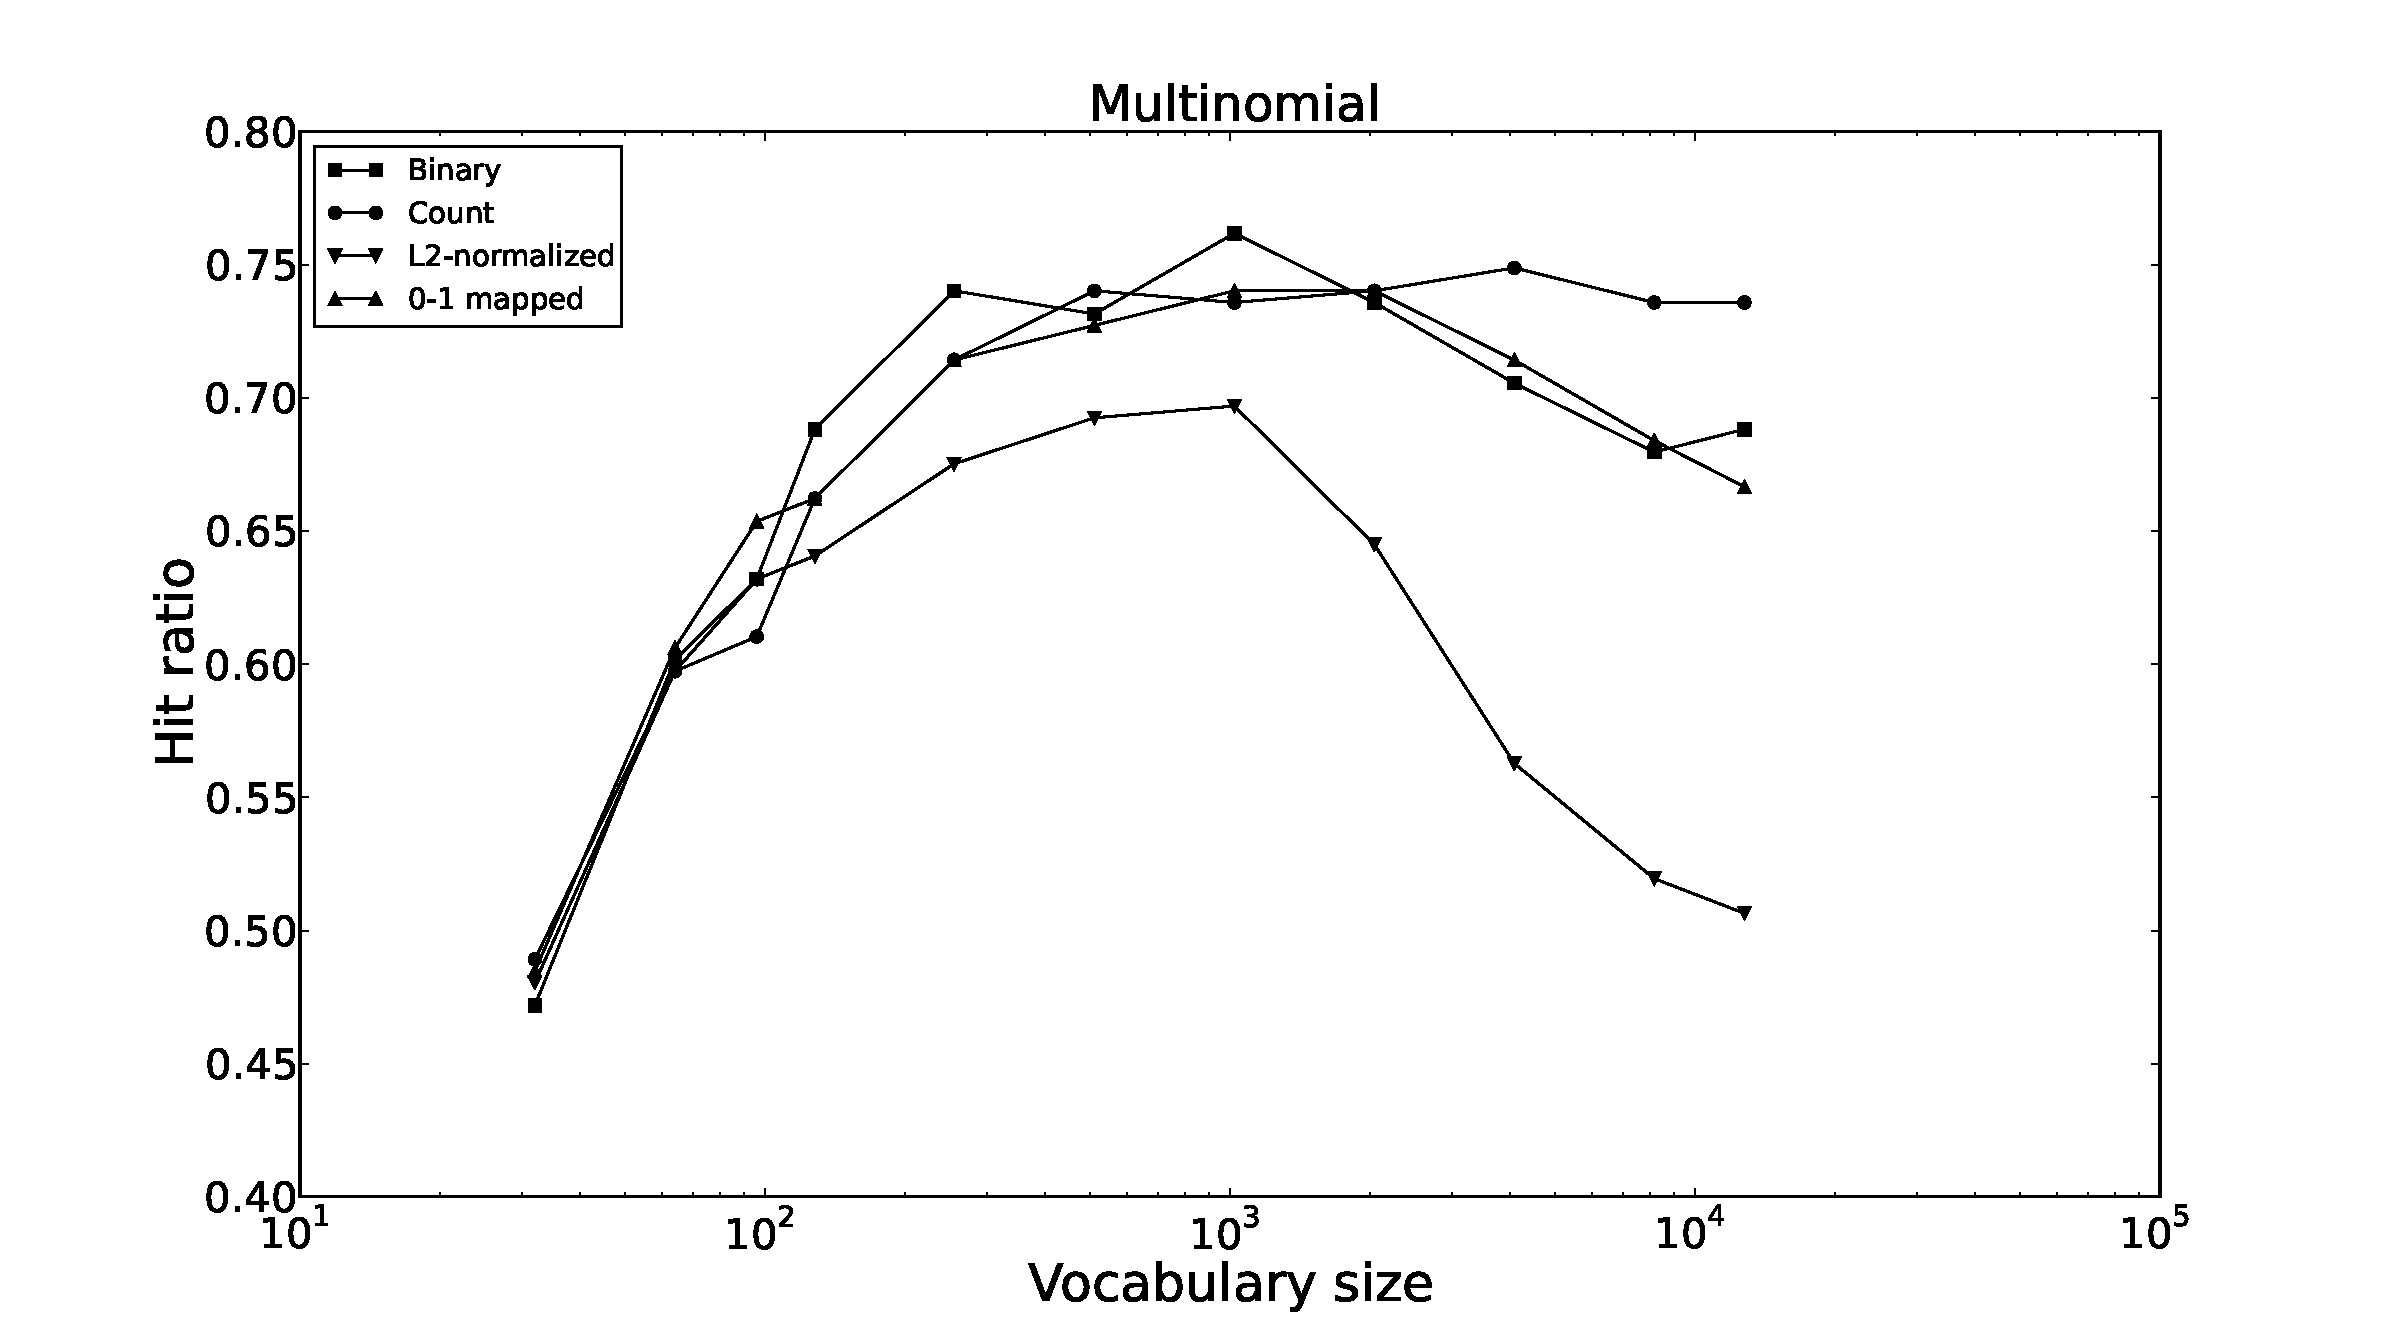
\includegraphics[width=\textwidth]{img/Multinomial-hitrate-eps-converted-to.pdf}
		\caption{Hit ratio of Multinomial classifier with varying vocabulary size.}
		\label{fig:hitrate-mn}
	\end{subfigure}
	\\
	\begin{subfigure}[b]{\figwidth}
		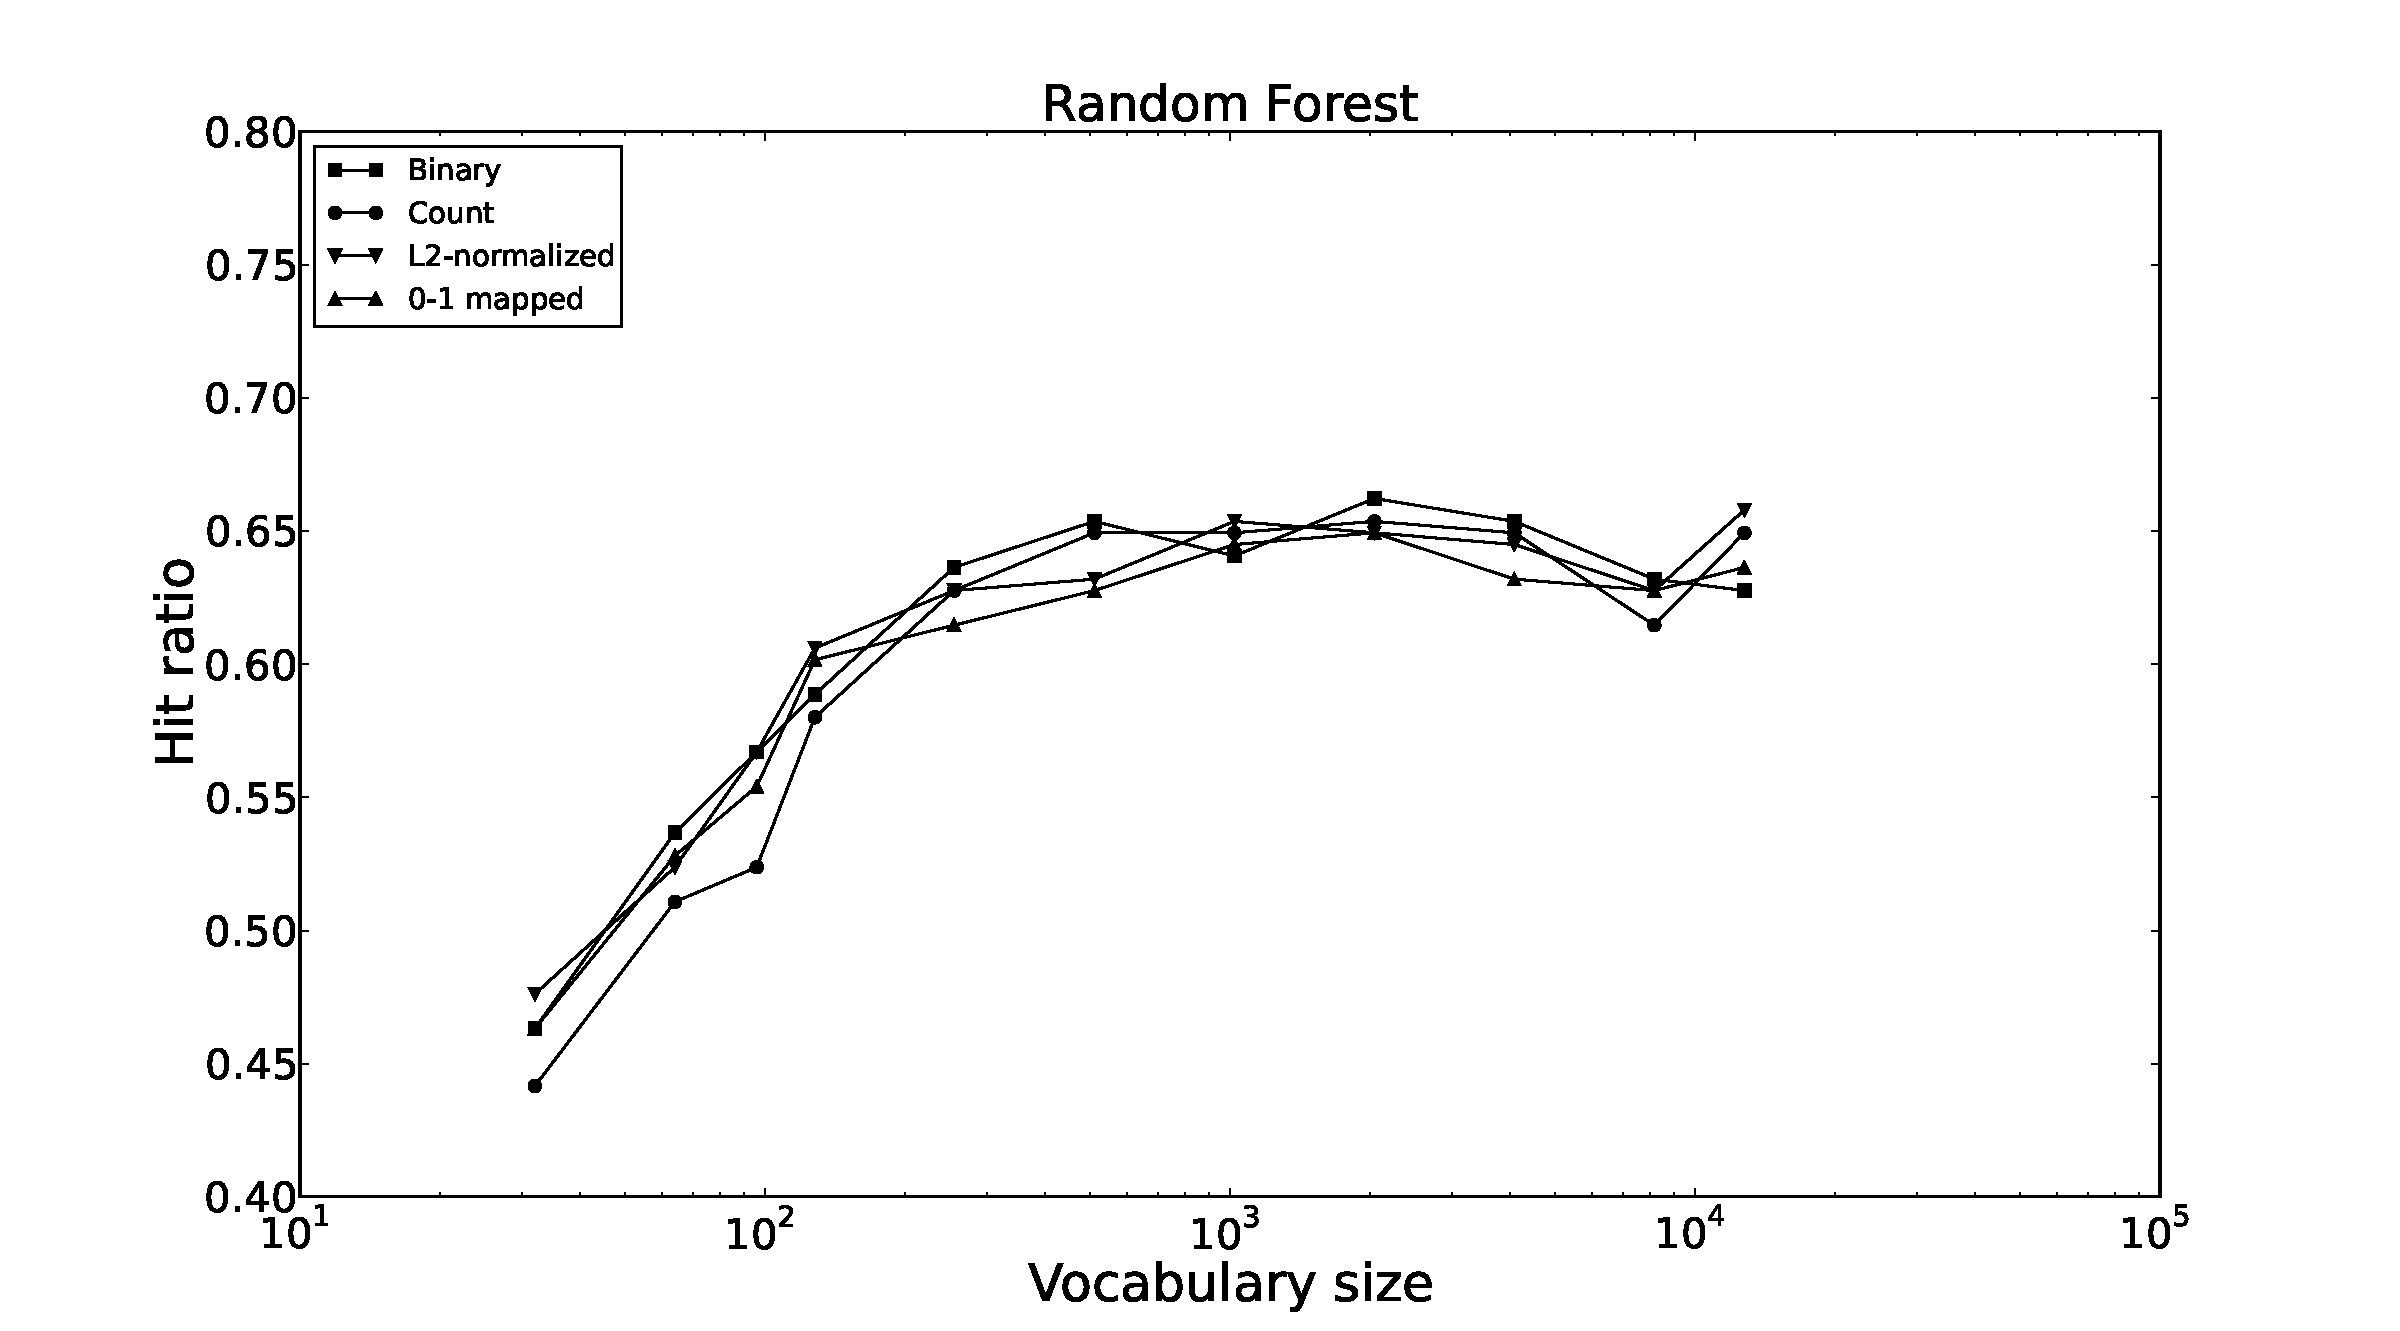
\includegraphics[width=\textwidth]{img/Random-Forest-hitrate-eps-converted-to.pdf}
		\caption{Hit ratio of Random Forest classifier with varying vocabulary size.}
		\label{fig:hitrate-rf}
	\end{subfigure}
	~
	\begin{subfigure}[b]{\figwidth}
		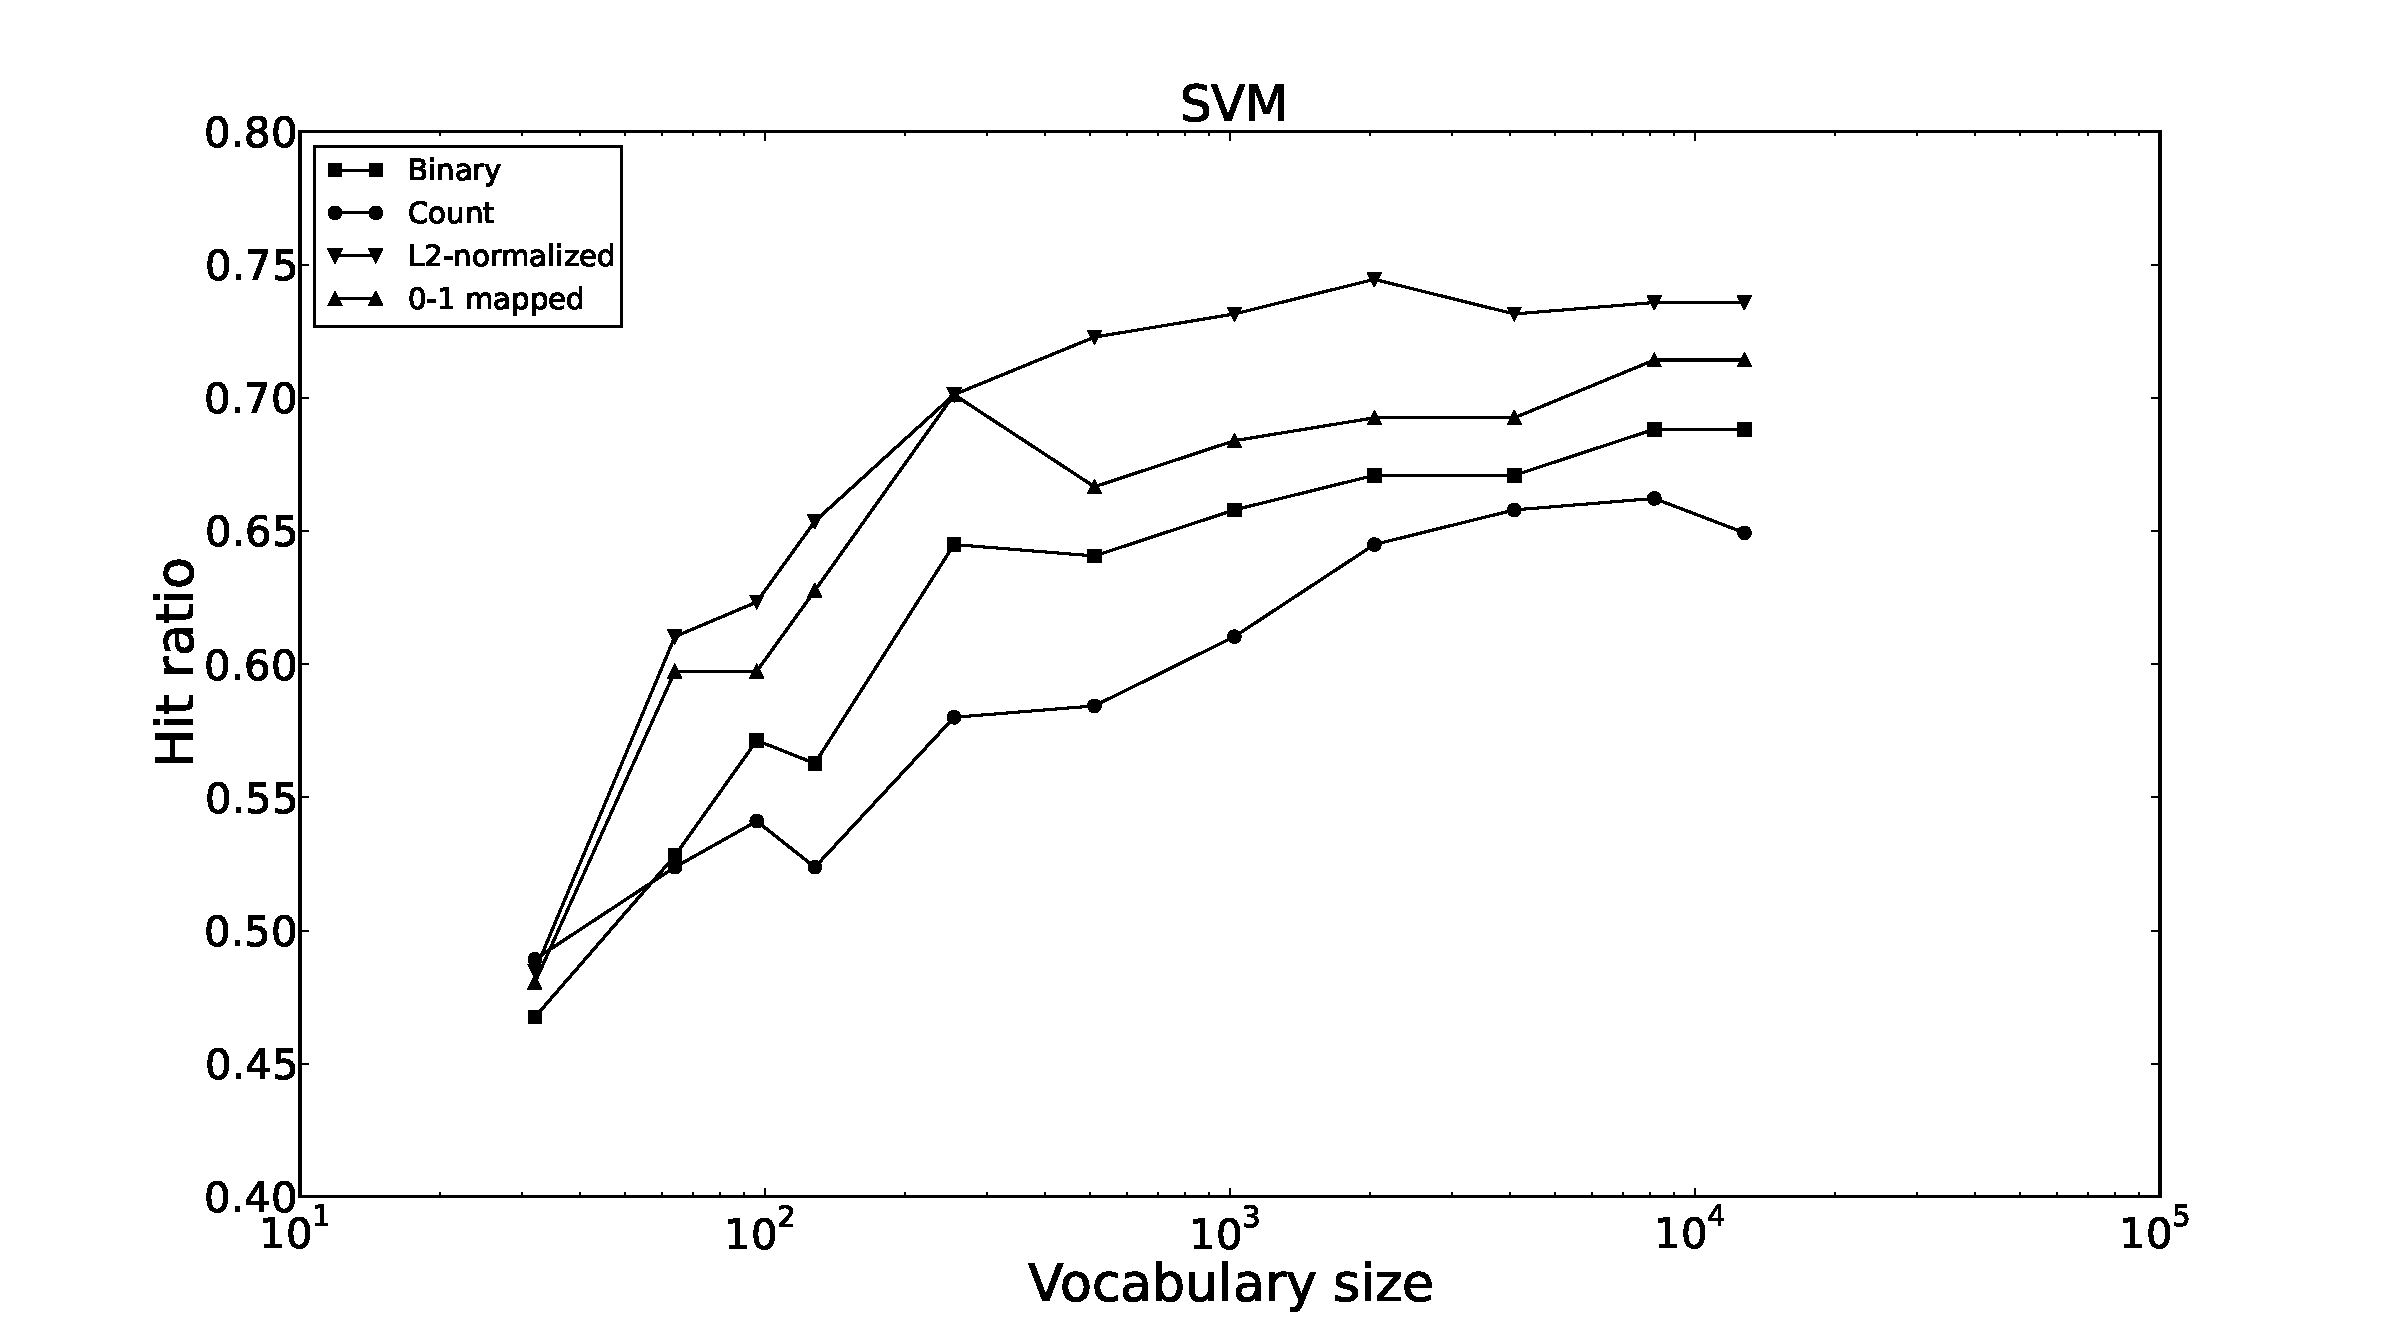
\includegraphics[width=\textwidth]{img/SVM-hitrate-eps-converted-to.pdf}
		\caption{Hit ratio of SVM classifier with varying vocabulary size.}
		\label{fig:hitrate-svm}
	\end{subfigure}
	\\
	\begin{subfigure}[b]{\figwidth}
		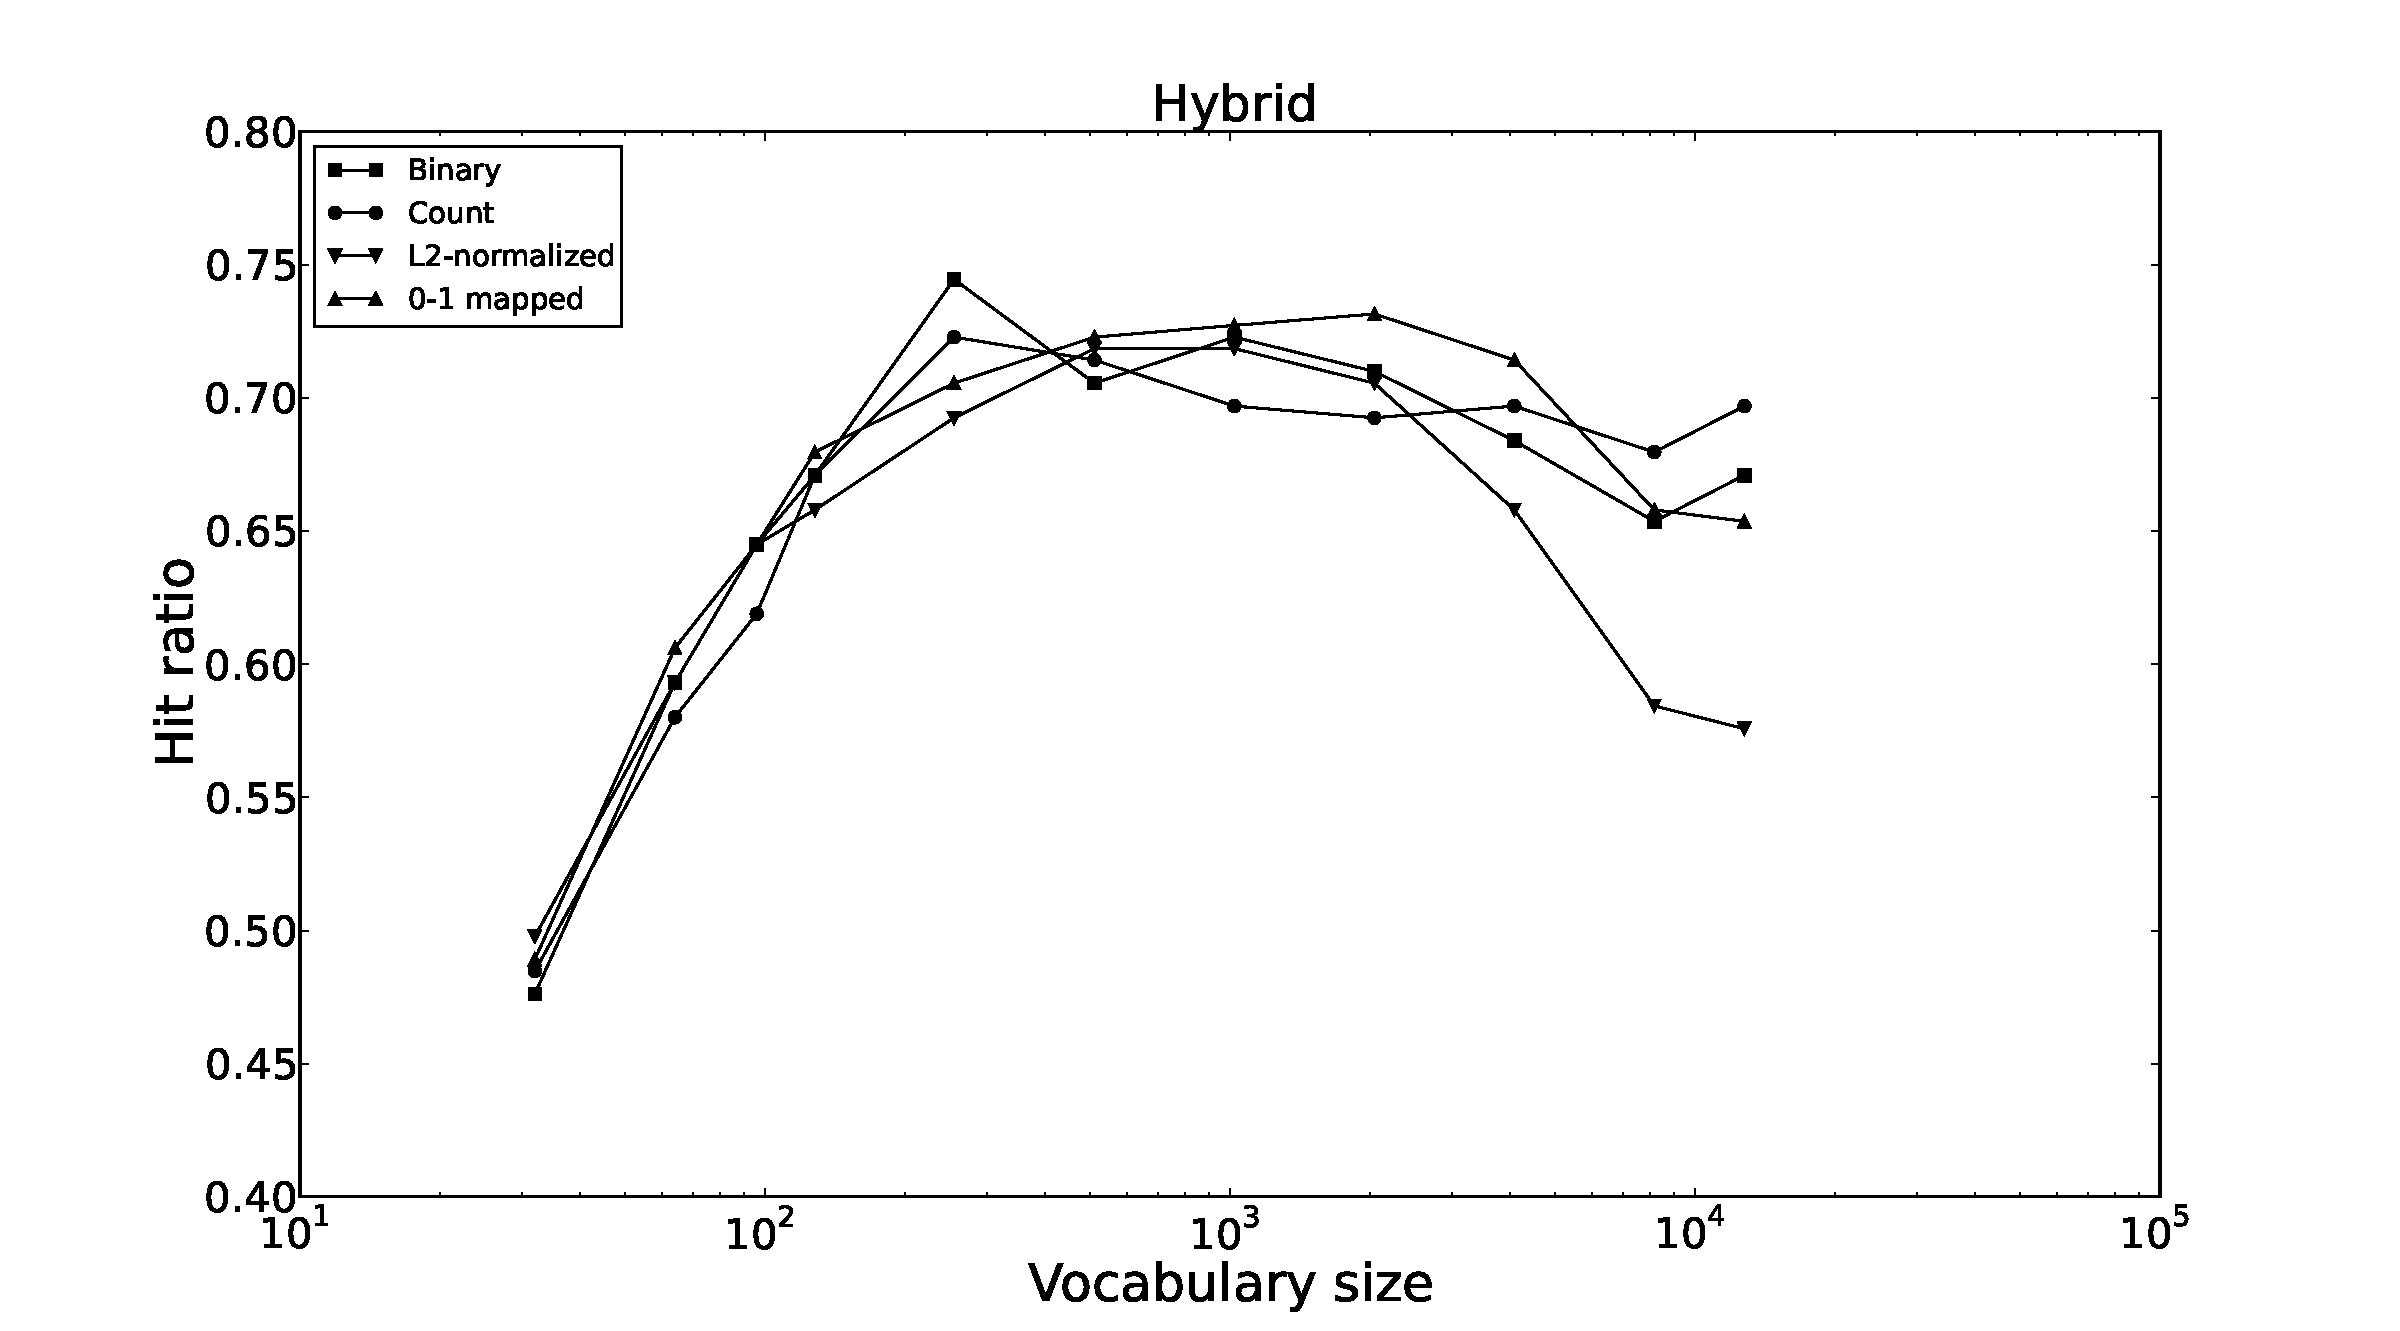
\includegraphics[width=\textwidth]{img/Hybrid-hitrate-eps-converted-to.pdf}
		\caption{Hit ratio of Hybrid classifier with varying vocabulary size.}
		\label{fig:hitrate-hybrid}
	\end{subfigure}
	\caption{Hit ratio vs vocabulary size}
	\label{fig:hitrate}
\end{figure}

